\documentclass[
  a4paper,
  12pt,
  oneside,
  parskip=half,
  listof=totoc,
  bibliography=totoc,
  DIV=12,
  numbers=noenddot,
  BA.tex
  ]{subfiles}

\begin{document}

\section{Quark-gluon plasma physics at colliders}

This chapter introduces the quark model and few aspects of quantum chromodynamics to then make the connection to emergent phenomena of QCD. It then describes how heavy ion collisions can be used to probe several aspects of the quark-gluon plasma, an emergent phenomenon. It also points out to experimental methods that can be used to study properties of the quark-gluon plasma. 

\subsection{The QGP as a quantum chromodynamics object}
In 1963, Gell-Mann and Zweig introduced quarks as elementary constituents of composite particles in need of a model that is able to explain the spectrum of strongly interacting particles \cite{peskin_introduction_2018}. In this model mesons are made up of quark-antiquark bound states while baryons are interpreted as bound states of three quarks, each chosen from a tuple of three possible quarks, up (u), down (d) and strange (s) which is the minimum number of quarks to explain already known quantum numbers and charges of hadrons. Three other quark species (flavors) have followed, namely charm (c), bottom (b) and top (t) in order to explain the discovery of additional hadrons. The charges of the quarks are fractional, they are $+2/3 \cdot e$ for (u,c,t) and $-1/3 \cdot e$ for (d,s,b) with the elementary charge $e$.

However, the quark model does not explain why no fractional charged particles are observed or that there is a baryon $\Delta^{++}$(uuu) with spin $3/2$ that has a fully symmetric wave function despite made up of quarks that are fermions and therefore obey Fermi-Dirac statistics \cite{peskin_introduction_2018}. The solution to this problem requires the introduction of another quantum number for quarks, namely the color charge, in which hadron wave functions must be antisymmetric in. There are three possible color charges for quarks ($i = 1,2,3$) that transform under the fundamental representation '$3$' of the $SU(3)_{C(olor)}$ symmetry while anti-quarks transform in the '$\bar{3}$' representation. The physics of color dynamics is called quantum chromodynamics (QCD). Under the postulate that all hadron wave functions are invariant under $SU(3)$ transformations, there are only few combinations allowed

\begin{equation}
	\bar{q}^i q_i \quad \epsilon^{ijk} q_i q_j q_k \quad \epsilon_{ijk} \bar{q}^i \bar{q}^j \bar{q}^k
\end{equation}

which are the wave functions of known light baryons and mesons \cite{peskin_introduction_2018}.

If one tries to separate a color-singlet state into colored components, for example by dissociating a meson into a quark and an antiquark, gluons, the quanta of the $SU(3)$ gauge field, form between the quark-antiquark pair \cite{peskin_introduction_2018}. These newly created gluons make the energy cost to separate them grow proportionally. This phenomenon is known as confinement of color and explains why no free quarks can be observed. At small length scales quarks interact only weakly in terms of the strong force and can be described as almost-free particles. This behavior is called asymptotic freedom.

In contrast to the description above it has been known since the 1970s that matter above some temperature and pressure scale, like present in the very early moments of our universe or in neutron stars, cannot be composed of individual hadrons \cite{collins_superdense_1975}. A neutron has a density of about $8 \cdot 10^{14} \frac{\text{g}}{\text{cm}^3}$, but the central density of a neutron star is ten to 100 times larger \cite{busza_heavy_2018}. Meaning that the hadrons inside of a neutron star must overlap, losing their individuality and making up a state of matter that is referred to as quark-gluon plasma (QGP). This form of matter must have had temperatures above the fundamental energy scale of quantum chromodynamics, which can be first-order approximated as the inverse of the size of a hadron. The QGP can be produced in heavy ion collisions, which is a powerful motivation to do heavy ion physics. Referring to \cite{anderson_more_1972} knowledge about QCD at the fundamental level does not guarantee insight into the systematics of such complex systems as the QGP. The system as a collection of well understood constituents itself makes insightful phenomena emerge. Figure \ref{fig:qcdphasediadram} shows the phase diagram of quantum chromodynamics. Lattice QCD calculations in thermal equilibrium show a continuous crossover around $T \approx 150 \bunit{MeV}$ for low $\mu_B$, the conditions in heavy ion collisions \cite{busza_heavy_2018}. It transitions from a hadron resonance gas at lower temperatures to QGP at higher temperatures. At higher $\mu_B$ the transition may become of first order at a critical point. Experimentally showing this critical point remains inconclusive. Interesting regions corresponding to the conditions in neutron stars and heavy ion collisions at various collider energies are marked in figure \ref{fig:qcdphasediadram}. 


\begin{figure}
	\centering
	\includegraphics[width=0.8\linewidth]{Media/Pictures/QCD_phase_diadram}
	\caption{The phase diagram of quantum chromodynamics. The diagram highlights naturally occurring regions like the one marking the conditions present in the early moments of the universe or in neutron stars (black). It also points out to regions that can be accessed artificially, for example at the Large Hadron Collider (pink) or at the accelerator complex FAIR that is currently under construction (brown). Image from \cite{gsi_helmholtzzentrum_fur_schwerionenforschung_gmbh_hot_nodate}.}
	\label{fig:qcdphasediadram}
\end{figure}

\subsection{Phenomenology of a heavy ion collision}

Let us now look at the current understanding of a heavy ion nuclei collision to gain an understanding of how they help us understand emergent phenomena of QCD. Lead nuclei are approximately spherical objects \cite{henderson_deformation_2025}. In the lab frame of a collider experiment beam nuclei appear as Lorentz-contracted discs as they move towards each other at speeds close to the speed of light \cite{busza_heavy_2018}. The thickness of the disc depends on the order of length contraction, so on the relativistic gamma factor $\gamma = (1-(v/c)^2)^{-1/2}$, its diameter is invariant under this Lorentz transformation. In the incoming nuclei gluons play a major role in the collision \cite{albacete_gluon_2014}. The gluons interact under extreme pressure and temperature and eventually thermalize into the QGP, a plasma with low specific shear viscosity, meaning it behaves like a perfect liquid \cite{busza_heavy_2018}. The specific shear viscosity is the ratio of the shear viscosity over the entropy density $\eta/s$. Although both numbers are exceedingly large, it is their ratio that is remarkably small. 

\begin{figure}
	\centering
	\begin{minipage}[t]{0.24\textwidth}
		1
		\includegraphics[width=\textwidth]{Media/Pictures/HeavyIonCollision_1}
	\end{minipage}
	\begin{minipage}[t]{0.24\textwidth}
		2
		\includegraphics[width=\textwidth]{Media/Pictures/HeavyIonCollision_2}
	\end{minipage}
	\begin{minipage}[t]{0.24\textwidth}
		3
		\includegraphics[width=\textwidth]{Media/Pictures/HeavyIonCollision_3}
	\end{minipage}
	\begin{minipage}[t]{0.24\textwidth}
		4
		\includegraphics[width=\textwidth]{Media/Pictures/HeavyIonCollision_4}
	\end{minipage}
	\caption{The simulated time evolution of two heavy ion nuclei (Au+Au) colliding at $200\bunit{GeV/c}$. \textbf{1} The Lorentz-contracted discs fly towards each other \textbf{2} At the time of collision, the energy density is the greatest, visualized through the red color \textbf{3} After the discs have passed each other, the hot QGP front continues propagating in beam direction, creating hadrons in its wake in the cooling zone \textbf{4} The hadrons can freely expand \linebreak The whole process from left to right takes about $40\bunit{fm/c}$. Images are snapshots from \cite{wit_busza_andre_yoon_yen-jie_lee_heavy_nodate}.}
	\label{fig:visualizationqgpproduction}
\end{figure}

Since the pressure is still high and the QGP can be described with relativistic hydrodynamics, the pressure-driven hydrodynamic expansion rapidly builds up large transverse velocities, so velocity components perpendicular to the beam axis, although they were small initially \cite{busza_heavy_2018}. A volume unit of QGP expands in all directions until the volume unit undergoes a phase transition according to the phase diagram of QCD shown in figure \ref{fig:qcdphasediadram}. This transition makes the fluid fall apart into individual hadrons. The time evolution of an exemplary heavy ion collision involving gold ions is shown in figure \ref{fig:visualizationqgpproduction}. Ultrarelativistic heavy ion collisions probe different aspects of QCD in their distinct evolutionary stages and are the only tool science has to test QCD and its emergent phenomena under extreme conditions in the laboratory \cite{busza_heavy_2018}.


\subsection{Particle jets as a probe of the QGP}

An important microscopic mechanism is the hard collision of individual partons in the incident nuclei. In hard collisions particles with large transverse momenta $p_T = \mathcal{O} (10\bunit{GeV/c})$ are produced, which are essential for analyzing the QGP's properties \cite{busza_heavy_2018}. The products can be traced back to the earliest moments of the collision where high-energy parton pairs and electroweak bosons are produced. They will then evolve, decay, radiate and therefore produce a cone-shaped spray of hadrons and high-energy photons, leptons or heavy $q\bar{q}$ pairs. This shower is also referred to as a jet \cite{busza_heavy_2018}. 

The high-$p_T$ partons traverse the QGP which is formed after the initial hard scattering took place. Therefore the energy and distribution of the jet constituents contain information about the produced QGP medium, like an X-ray scan, having documented how jet constituents have lost energy in the medium or, on the other hand, influence the medium itself \cite{busza_heavy_2018}. To extract this information one needs to exactly know how jets behave in a non-QGP environment, for example in pp collisions. The production of hard, meaning high-$p_T$ $\gamma$ and $Z^0$, has been studied in pp and A--A (heavy ion) collisions thoroughly \cite{collaboration_measurement_2013} \cite{collaboration_study_2015} \cite{collaboration_centrality_2016}. The measured production rates of colorless hard probes in A--A heavy ion collisions align with the production rate in pp collisions, multiplied with the number of nucleon interactions that happen during the overlap when the nuclei pass by. This underlies small corrections because the nucleons are inside of the nuclei. Since the QGP is a QCD object and $\gamma$ and $Z^0$ are colorless, they are not affected by the post-collision A--A environment. On the other hand, strongly interacting, colored, hard probes like jets of high transverse momentum (high $p_T$) hadrons, heavy quarks and so on, can be used to compare A--A to pp collisions to investigate how they are modified by the QGP medium. Experimental measurements of jets, high-$p_T$ hadrons and heavy quarks coming from jets \cite{connors_review_2018} have shown that jets lose a noticeable amount of energy as they propagate through the QGP, with the energy ending up as many soft particles moving at large angles relative to the jet axis \cite{collaboration_measurement_2016}. When particles travel at a speed faster than the velocity of sound in a medium, like an aircraft flying at supersonic speed, they generate Mach waves that can add up to a shockwave, called the Mach cone \cite{sasoh_compressible_2020}. Hydrodynamic simulations of the QGP have shown that such Mach cone can also be produced inside the QGP by propagating jets \cite{casalderrey-solana_conical_2005}. The study of such a QGP Mach cone can provide important information about the properties of the QGP, such as transport coefficients or the equation of state \cite{yang_3d_2023}. However, this Mach cone has never been observed unambiguously because when averaging the soft Mach cone particles over their possible propagation angles, their distribution becomes indifferent from that of soft hadrons from jet fragmentation \cite{chen_effects_2018} \cite{chen_search_2021}.

The collection of such phenomena is called "jet quenching" and makes up a very important part of QGP studies, as they give us direct evidence of strong interactions between the jet and the liquid \cite{busza_heavy_2018}.

\pagebreak

\subsection{The diffusion wake}

\begin{mdframed}
	\textbf{Definition (Pseudo-)rapidity/Azimuth angle:} \textit{The pseudorapidity is defined as $\eta \equiv - \log(\tan(\theta/2))$ where $\theta$ is the polar angle in momentum space relative to the beam direction. $\eta$ is related to the rapidity $y$ with $\eta = y$ for massless particles \cite{busza_heavy_2018}. \\ The azimuth angle $\phi$ is the polar angle along the circumference of the detector barrel and has values of $-\pi \leq \phi \leq \pi$.}
	\begin{figure}[H]
		\centering
		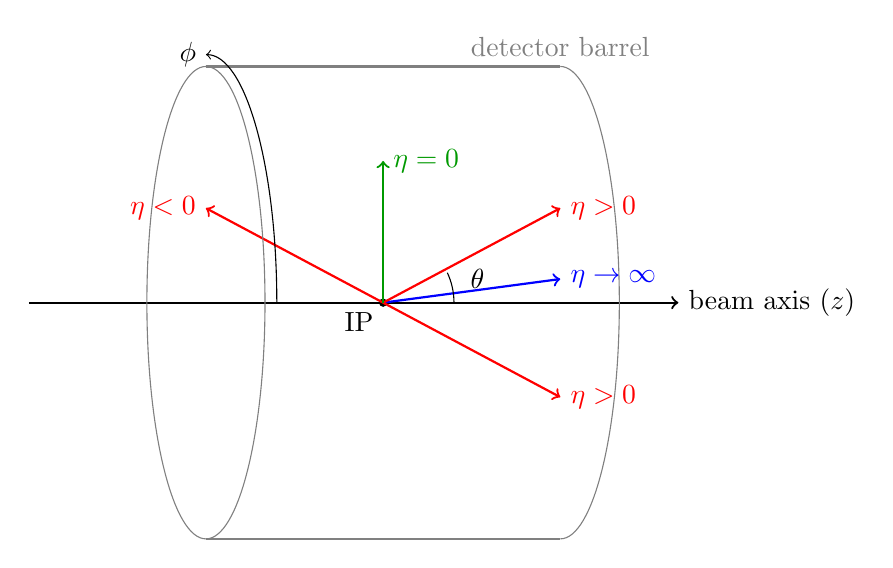
\begin{tikzpicture}[scale=1.5]
			
			% Beam-Achse (z-Achse)
			\draw[->, thick] (-3,0) -- (2.5,0) node[right] {beam axis ($z$)};
			
			% Wechselwirkungspunkt
			\filldraw[black] (0,0) circle (0.03) node[below left] {IP};
			
			% Teilchenspuren
			\draw[->, thick, blue] (0,0) -- (1.5,0.2) node[right] {$\eta \rightarrow \infty $};
			\draw[->, thick, red] (0,0) -- (1.5,0.8) node[right] {$\eta > 0$};
			\draw[->, thick, red] (0,0) -- (1.5,-0.8) node[right] {$\eta > 0$};
			\draw[->, thick, red] (0,0) -- (-1.5,0.8) node[left] {$\eta < 0$};
			\draw[->, thick, green!60!black] (0,0) -- (0.0,1.2) node[right] {$\eta = 0$};
			
			%Detector barrel
			\draw[gray](-1.5,0) ellipse (0.5 and 2.00);
			\draw[thick, gray] (-1.5, 2.0) -- (1.5, 2.0) node[above] {detector barrel};
			\draw[thick, gray] (-1.5, -2.0) -- (1.5, -2.0);
			\draw[gray](1.5,-2) arc(-90:90:0.5 and 2);
			
			%phi labeling
			%\draw[->, thick] (-1.5,0) -- (-1.2, );
			%\draw[thick] (-3,0) -- (-2.75, 0.0) node[right] {$\phi = 0$};
			\draw[black, ->](-0.9,0) arc(0:90:0.6 and 2.1) node[left] {$\phi$};
			
			% Winkelmarkierung (Theta)
			\draw (0.6,0) arc[start angle=0,end angle=25,radius=0.6];
			\node at (0.8,0.2) {$\theta$};
			
		\end{tikzpicture}
		\label{fig:pseudorapidity}
	\end{figure}
	
\end{mdframed}

Shock waves that form a Mach cone in the quark-gluon plasma are always accompanied by a diffusion wake behind the propagating jet as a hydrodynamic effect of the medium response to the energy-momentum deposition \cite{neufeld_mach_2009} \cite{ke_qgp_2021}. The diffusion wake emerges because the thermal medium parton density is depleted behind the propagating jet partons \cite{he_linear_2015}. A direct consequence of such a diffusion wake is the depletion of soft hadrons in the final hadron spectra in the opposite direction to the propagating jet \cite{chen_search_2021}.

The terminology of opposite direction may lead to confusion and it should be clarified what is meant. When a jet has a certain rapidity and azimuthal angle $(\phi_\text{jet}, \eta_\text{jet})$, the postulated particle depletion is exactly opposite in azimuthal angle, but has the same rapidity, so $(\phi_\text{depletion}, \eta_\text{depletion}) = (\phi_\text{jet} \pm \pi, \eta_\text{jet})$. The reasoning why rapidity is not also inverted becomes clear when boosting into the reference system of the jet along the beam axis. Now the jet has a rapidity of zero and is perpendicular to the beam axis. The depletion of soft particles is consequently at a rapidity of zero. When boosting back into the lab system the depletion has the same rapidity as the jet.

Although no other medium effect competes with the diffusion wake signal, it can still be overwhelmed by other effects \cite{chen_effects_2018}\cite{collaboration_using_2022}\cite{chen_search_2021} making it difficult to measure. Anisotropies in per-event charged hadron momentum distributions in the $(\phi, \eta, p_T)$ is one of such diffusion wake overwhelming effects. Further details are discussed as anisotropic flow in chapter \ref{sec:analysis-of-heavy-ion-collision-data}. One major challenge while searching for the jet-induced diffusion wake is to distinguish between particles produced by the jet-induced medium response and those originating from jet hadronization and the underlying QGP background \cite{yang_background-free_2025}. There have been measurements on the diffusion wake using different methods to overcome these difficulties. The CMS collaboration \cite{collaboration_evidence_2026} has identified $Z^0$ bosons via their $\mu^+ \mu^-$ decay channel. Measurements of any jets produced in the same hard scattering as these bosons offer a controlled configuration for the initial hard scattering \cite{brewer_disentangling_2022} \cite{wang_study_1997} \cite{wang_jet_1996} \cite{kartvelishvili_z_1995}. The transverse momentum  of the electroweak boson reflects the initial energy of the associated parton before any medium-induced energy loss occurs \cite{kang_vector_2017} \cite{dai_momentum_2013}, meaning that the $Z^0$ boson is reflected opposite to the jet of interest. The diffusion wake is therefore measured in the correlation of charged hadrons in the azimuthal direction of the $Z^0$ boson. Background is subtracted using a mixed-event method.

\begin{mdframed}
	\textbf{Definition Mixed Event Method:} \textit{In heavy ion analyses, the mixed-event method estimates the uncorrelated combinatorial background by constructing pairs from particles taken from different collision events. Since particles from different events have no physical correlation with each other, the resulting distribution retains effects such as detector acceptance and single-particle kinematics but largely removes genuine two-particle correlations \cite{alice_collaboration_multiplicity_2016}.}
\end{mdframed}

One major flaw of the $Z^0$ boson analysis is that because of particle number conservation, the mixed-event method produces a negative $Z^0$ hadron correlation in the direction of the $Z^0$ \cite{yang_background-free_2025}. Although the shape of such negative correlation is very different to that of the searched diffusion wake, this may lead to questions about the genuineness of the observed diffusion wake signal. The results of the $Z^0$ boson study are shown in figure \ref{fig:cmsdiffwakezboson}.

\subsection{Theoretical proposal: Use dijets to measure the diffusion wake}

In \cite{yang_background-free_2025} it was recently proposed a method to isolate the jet-induced diffusion wake signal from the underlying background using dijet events. At leading order two correlated jets are produced back-to-back due to conservation of momentum in azimuthal angle ($\Delta \phi = \pi$). Deviations come primarily from soft gluon radiation in the region of $\Delta \phi = \pi$, meaning this is an effect of higher-order QCD radiation \cite{martinez_azimuthal_2022} .
The method works without depending on the limited availability of $Z^0/\gamma$-jet events and removes the need for special detector requirements and background subtractions. The analysis has shown the rapidity correlations of soft hadrons relative to the leading jet become strikingly asymmetric when comparing events with no/small and large dijet rapidity gaps, \cite{yang_rapidity_2025} offering unambiguous evidence for the presence of the diffusion wake in dijet events. The method studies the correlation of soft hadrons behind the subleading jet, so the jet with less transverse momentum of the two. Consequently, the focus lies on the diffusion wake of the subleading jet. The subleading jet has less transverse momentum and has therefore deposited more momentum in the QGP.  When the subleading jet has the same rapidity as the leading jet, its diffusion wake is covered by the leading jet. If on the other hand the subleading jet has another rapidity than the leading jet, its diffusion wake is visible next to the leading jet (see figure \ref{fig:DijetProposal2} (a)) Hadron correlations showcasing small as well as large rapidity gaps for pp and Pb--Pb simulations are shown in figure \ref{fig:DijetProposal}. The result (figure \ref{fig:DijetProposal2} (c)) is close to background-free, because the QGP background is unaffected by the rapidity gap apart from small effects \cite{yang_background-free_2025}.

\begin{figure}
	\centering
	\includegraphics[width=0.8\linewidth]{Media/Pictures/DijetProposal_1.png}
	\caption{ a) Wake-front (red-yellow-green), diffusion wake (blue) and induced gluon radiation in dijet events in heavy ion collisions. b) Illustration of the effect of the diffusion wake (dashed) from one jet on the jet-hadron correlation in the other jet with (red) and without (blue) a rapidity gap and c) the rapidity asymmetry of their difference. From \cite{yang_rapidity_2025}.}
	\label{fig:DijetProposal2}
\end{figure}

A simulation of dijet events with the CoLBT-hydro model \cite{yang_background-free_2025} has also been conducted by theoreticians. CoLBT-hydro is used to simulate the transport of the dijets in the QGP and also to calculate the rapidity asymmetry in central 0--10\% collisions at $\sqrt{s_{NN}} = 5.02\bunit{TeV}$. The leading and subleading jet must have transverse momenta of more than $120\bunit{GeV/c}$ and $90\bunit{GeV/c}$ and a separation in pseudorapidity of $|\Delta \eta_{\text{Leading} , \text{Subleading}}| < 1.6$. Furthermore, the jets are required to be almost back-to-back in azimuthal angle, imposed by $|\Delta \phi_{\text{Leading}, \text{Subleading}}| > \pi/2$. Low-$p_T$ hadrons are studied on the near-side of the leading jet, meaning that the separation of hadrons and the leading jet is $\Delta \phi_{\text{Leading} , h} < \pi/2$. The leading jet is required to be in the positive pseudorapidity range, so $\eta_{\text{Leading}} > 0$. If not, the whole event is mirrored at the $\eta = 0$ plane. Events are divided into two classes depending on the configuration of the two jets in pseudorapidity: (1) $\eta_{\text{Leading}} \cdot \eta_{\text{Subleading}} > 0$ for two jets in the same hemisphere and (2) $\eta_{\text{Leading}} \cdot \eta_{\text{Subleading}} < 0$ for two jets in opposite hemispheres with a large dijet rapidity gap \cite{yang_background-free_2025}. We call the two cases large/small rapidity gaps to be consistent with \cite{yang_background-free_2025}. It is nevertheless important to notice that case (2) does not necessarily impose a large dijet rapidity gap, best demonstrated on the example where the two jets have the pseudorapidities $\eta_{\text{Leading}} := \epsilon, \eta_{\text{Subleading}} := -\epsilon$, in which case the jets are merely separated, but $\eta_{\text{Leading}} \cdot \eta_{\text{Subleading}} < 0$. On average though, the separation is greater than in case (1).

\begin{figure}[H]
	\centering
	\includegraphics[width=0.9\linewidth]{Media/Pictures/DiffusionWakeSimu}
	\caption{Rapidity asymmetry between soft hadron rapidity distributions in the direction of the leading jet ($\Delta \phi_{\text{Leading,h}} < \pi/2$) in two different classes of dijets: (1) $\eta_{\text{Leading}} \cdot \eta_{\text{Subleading}} > 0$ and (2) $\eta_{\text{Leading}} \cdot \eta_{\text{Subleading}} < 0$, for $p_T^\text{h} \in [1.0, 2.0] \bunit{GeV/c}$ (black lines with gray bands) and $p_T^\text{h} \in [2.0, 4.0] \bunit{GeV/c}$ (blue lines with blue bands). The left panel is for 0--10\% Pb--Pb collisions and the right panel has the pp baseline subtracted. The label Leading/Subleading is equivalent to jet$_1$/jet$_2$ in the figure and was adapted for readability reasons. From \cite{yang_background-free_2025}.}
	\label{fig:diffusionwakesimu}
\end{figure} 

The results of the simulation are shown in figure \ref{fig:diffusionwakesimu}. The depletion can be seen in the negative pseudorapidity range for soft hadrons. The leading jet is fixed at positive pseudorapiditiy and the subleading jets, having a negative pseudorapidity, produces a depletion of soft hadrons in the negative pseudorapidity range, azimuthally next to the leading jet. It is the goal of the following chapters to study possible biases that could contribute to such a signal or oppose it and to measure the diffusion wake in experimental data with different analysis methods.



\end{document}